\documentclass{sig-alternate}

\usepackage[utf8]{inputenc}
\usepackage[T1]{fontenc}
\usepackage{graphicx}
\usepackage{amssymb}
\usepackage{amsmath}
\usepackage{mysymbols}
\usepackage{hyperref}
\usepackage{tikz}

\usepackage{xcolor}
\newcommand{\todo}[1]{\textcolor{red}{(#1)}}

\newcommand{\Cyc}{\Phi}  % Cyclotomic polynomial

\begin{document}

\title{Cool title to catch Lenstra's eye goes here}
\numberofauthors{3}
\author{
  \alignauthor Luca De Feo
  \alignauthor Javad Doliskani
  \alignauthor Éric Schost
}

\maketitle
\begin{abstract}
  We build towers.
\end{abstract}
\category{F.2.1}{Theory of computation}{Analysis of algorithms and problem complexity}[Computations in finite fields]
\category{G.4}{Mathematics of computing}{Mathematical software}
\terms{Algorithms,Theory}
\keywords{Finite fields, irreducible polynomials, extension towers, algebraic tori, elliptic curves.}

%%%

\section{Introduction}
\label{sec:intro}

Building arbitrary finite extensions of finite fields is a fundamental
task in any computer algebra system. Disregarding generic solutions
using multivariate algebra and Grobner bases, most systems are limited
to construct extensions of prime fields. There is one notable
exception: Magma~\cite{MAGMA} has implemented for a long time a
powerful system of ``compatibly embedded finite
fields''~\cite{bosma+cannon+steel97}, capable of building extensions
of any finite field and taking track of the embeddings between the
fields.

The system implemented in Magma, as described in the original paper,
uses linear algebra to describe the embeddings of finite fields. From
a complexity point of view this is far from optimal, indeed one may
hope to compute and apply the morphisms in (quasi)-linear time (in the
degree of the extension). Even worse, the quadratic memory
requirements make the system unsuitable for embeddings of large degree
extensions. Although the Magma core has evolved since the publication
of the paper, our experiments in Section~\ref{sec:bench} show that
embeddings of large extension fields are still out of reach in Magma.

In this paper we propose an approach based on polynomial arithmetic
rather than linear algebra, yielding much better performances. Our
solution only applies to some special cases, but we hope that it will
pave the way towards a complete solution. The technique we present is
similar to the one in~\cite{df+schost12} in that we construct families
of irreducible polynomials with special properties, then give
algorithms (called \emph{lift} and \emph{push}) that exploit the
special form of those polynomials to apply the embeddings. The
families of polynomials we use come from work of Lenstra and De Smit
on the algebraic closure of finite
fields~\cite{lenstra+desmit08-stdmodels}, and from work of Couveignes
and Lercier on constructing irreducible polynomials in quasi-linear
time~\cite{couveignes+lercier11}.

The focus of this paper is on the representation of extensions of
\emph{large} degree and their embeddings. We do not consider issues
related to special representations of small finite fields, such as
primitive polynomials, Zech logarithms, Conway polynomials, etc. A
user doing computations in a single, fixed, extension field will
clearly benefit more from these optimizations than from our
construction. However, a variety of computations in number theory and
algebraic geometry requires frequently constructing new extension
fields and moving elements from one to the other. Examples of these
algorithms are~\cite{df10} \todo{cite more}. Our construction makes
them feasible for much larger sizes than it was previously possible.

This paper is organized as follows. \todo{How?}

%%%

\section{Finite fields and embeddings}
\label{sec:finite-field-embedd}
We fix the following notation: $p$ is a prime, $d$ a positive integer,
$q=p^d$, $\F_p$ and $\F_q$ are the finite fields with $p$ and $q$
elements respectively.

The field $\F_q$ can be constructed as the splitting field of any
irreducible polynomial of degree $d$, we call this the \emph{defining
  polynomial} of $\F_q$. There are about $p^d/d$ such irreducible
polynomials over $\F_p$ \todo{cite something}, giving as many
different ways of representing $\F_q$. Furthermore, there is no
canonical way of establishing isomorphisms between them, indeed a
field with $p^d$ elements has $d$ automorphisms fixing $\F_p$.

A field with $p^d$ elements contains subfields with $p^n$ elements for
any $n|d$. For the same reasons as above, there is no canonical way of
embedding one finite field into another.

Let $\ell$ be another integer. We define the \emph{$\ell$-adic
  closure} of $\F_p$ as follows. Fix arbitrary embeddings
\begin{equation*}
  \F_p \subset \F_{p^\ell} \subset \F_{p^{\ell^2}} \subset \cdots,
\end{equation*}
the $\ell$-adic closure is the infinite field defined by
\begin{equation*}
  \F_p^{(\ell)} = \bigcup_{i>0}\F_{p^{\ell^i}}.
\end{equation*}
When $\ell$ is prime, the Galois group of $\F_p^{(\ell)}/\F_p$ is a
procyclic group isomorphic to $\Z_\ell$, the $\ell$-adic integers. Let
$\bar{\F}_p$ be an algebraic closure of $\F_p$, then there is a well
known isomorphism
\begin{equation}
  \label{eq:tensor}
  \bar{\F}_p \isom \bigotimes_{\ell\text{ prime}} \F_p^{(\ell)},
\end{equation}
where the tensor products are over $\F_p$.

A \emph{root of unity} is an element of finite multiplicative order;
the element is said to be a \emph{$n$-th root} if this order divides
$n$, a \emph{primitive $n$-th root} if it is exactly $n$. Obviously,
every element of a finite field is a root of unity. The $n$-th
cyclotomic polynomial $\Cyc_n$ is the polynomial whose roots are the
primitive $n$-th roots of unity. It has integer coefficients and its
degree is $\euler(n)$. Viewed as a polynomial with coefficients in $\F_q$,
it splits into irreducible factors of degree equal to the order of $q$
in $\Z/n\Z$, and splits completely in an extension of the same
degree. We call this splitting field the $n$-th Kummer extension of
$\F_q$.

Most computer algebra systems construct the field $\F_q$ by taking
degree $d$ polynomials at random until one irreducible is found. This
approach has a cost at least quadratic in the degree $d$. More
advanced constructions use Eq.~\eqref{eq:tensor}: they factor $d$ into
prime powers, for each prime power construct an extension of $\F_p$ of
that degree, then glue all the extensions together by taking
\emph{composita}.

The classical way of taking \emph{composita} is \todo{what?}

\begin{figure}
  \centering
  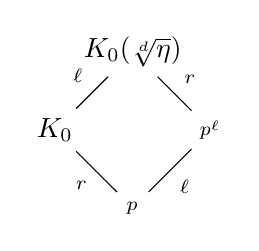
\begin{tikzpicture}[node distance=1.4cm]
    \node(Fp){$\F_p$};
    \node(K0)[above left of=Fp]{$K_0$};
    \node(K1)[above right of=K0]{$K_0(\sqrt[d]{\eta})$};
    \node(Fq)[above right of=Fp]{$\F_{p^\ell}$};
    \draw (Fp) edge node[auto]{\scriptsize$r$} (K0)
               edge node[auto,swap]{\scriptsize$\ell$} (Fq)
          (K1) edge node[auto,swap]{\scriptsize$\ell$} (K0)
               edge node[auto]{\scriptsize$r$} (Fq);
  \end{tikzpicture}
  \caption{Shoup's construction}
  \label{fig:shoup}
\end{figure}

Algorithms to construct extensions of degree a prime power can be
thought of as constructions for $\ell$-adic closures of
$\F_p$. Shoup's~\cite{shoup94} is summarized in
Figure~\ref{fig:shoup}. Let $\ell$ be a prime, the algorithm starts by
constructing $K_0$ the $\ell$-th Kummer extension of $\F_p$, then
looks for a non $\ell$-adic residue $\eta$ and uses it to construct a
degree $\ell$ extension $K_1$. This last step can be repeated several
times, to obtain an extension of degree $\ell^i$ of $K_0$. Finally it
takes the trace of a random element of $K_1$ down to $\F_{p^\ell}$ and
computes its minimal polynomial over $\F_p$, which is very likely to
be a defining polynomial for $\F_{p^\ell}$. Unless $K_0$ equals $F_p$,
Shoup's construction has quadratic complexity in $\ell$.  Couveignes
and Lercier give an alternative construction with complexity
subquadratic in $\ell$~\cite{couveignes+lercier11}; we will discuss it
in Section~\ref{sec:fibers}.


%%%

\section{Lenstra's and De Smit's tower}
\label{sec:LDtower}

Shoup's construction is non-deterministic, and it is shown that any
degree $\ell$ irreducible polynomial can be obtained that way. We now
describe a deterministic variant of Shoup's construction given by
Lenstra and De Smit~\cite{lenstra+desmit08-stdmodels}.

\begin{figure}
  \centering
  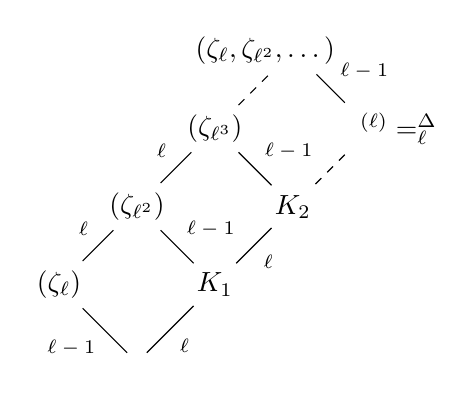
\begin{tikzpicture}[node distance=1.4cm]
    \node(Q){$\Q$};
    \node(Q0)[above left of=Q]{$\Q(\zeta_\ell)$};
    \node(K1)[above right of=Q]{$K_1$};
    \node(Q1)[above right of=Q0]{$\Q(\zeta_{\ell^2})$};
    \node(K2)[above right of=K1]{$K_2$};
    \node(Q2)[above right of=Q1]{$\Q(\zeta_{\ell^3})$};
    \node(Koo)[above right of=K2]{$\qquad \Q^{(\ell)} = \Q_\ell^\Delta$};
    \node(Qoo)[above right of=Q2]{$\Q(\zeta_\ell,\zeta_{\ell^2},\dots)\qquad$};
    \draw (Q) edge node[auto]{\scriptsize$\ell-1$} (Q0)
              edge node[auto,swap]{\scriptsize$\ell$} (K1)
          (K1) edge node[auto,swap]{\scriptsize$\ell-1$} (Q1)
               edge node[auto,swap]{\scriptsize$\ell$} (K2)
          (Q1) edge node[auto,swap]{\scriptsize$\ell$} (Q0)
          (Q2) edge node[auto]{\scriptsize$\ell-1$} (K2)
               edge node[auto,swap]{\scriptsize$\ell$} (Q1)
               edge[dashed] (Qoo)
          (Koo) edge[dashed] (K2)
               edge node[auto,swap]{\scriptsize$\ell-1$} (Qoo);
  \end{tikzpicture}
  \caption{The $\ell$-adic extension of $\Q$.}
  \label{fig:ladic}
\end{figure}

From now on, let $\ell$ be a prime different from the characteristic
$p$. For simplicity, we suppose $\ell\ne2$. Let $\zeta_{\ell^i}$ be
primitive $\ell^i$-th roots of unity such that
$\zeta_{\ell^i}^\ell=\zeta_{\ell^{i-1}}$. Consider the tower of
extensions of the rationals given by
\begin{equation*}
  \Q \subset \Q(\zeta_\ell) \subset \Q(\zeta_{\ell^2}) \subset \cdots,
\end{equation*}
its limit is an infinite extension with Galois group isomorphic to
$\Z_\ell^\ast\isom\Delta\times\Z_\ell$, where $\Delta$ is the torsion
part of $\Z_\ell^\ast$, a cyclic group of order $\ell-1$. The
\emph{$\ell$-adic extension of $\Q$} is defined as the subfield fixed
by $\Delta$:
\begin{equation}
  \label{eq:}
  \Q^{(\ell)} = \Q(\zeta_\ell, \zeta_{\ell^2}, \dots)^\Delta,
\end{equation}
it is the unique extension of the rationals having $\Z_\ell$ as Galois
group~\cite{lang1990cyclotomic,washington1997introduction}. The
construction of $\Q^{(\ell)}$ is summarized in
Figure~\ref{fig:ladic}. If we replace $\Q$ with a number field, we
obtain what is called the \emph{canonical $\ell$-adic extension}; its
Galois group is still $\Z_\ell$, but now there are others with this
property.

The cyclotomic extensions used to construct $\Q^{(\ell)}$ are
integral, thus it makes sense to reduce them modulo $p$. It turns out
that the reduction modulo $p$ of $\Q^{(\ell)}$ is an $\ell$-adic
closure of $\F_p$. Using number fields, this can be easily generalized
to build the $\ell$-adic closure of $\F_q$. We give two examples of
this construction.

\paragraph{$T_1$-extensions}

\paragraph{$T_2$-extensions}



%%%

\section{Towers from irreducible fibers}
\label{sec:fibers}
Interpreting the primitive roots tower and the LD-tower as fibers of
$T_1$ and $T_2$ respectively. Using elliptic curves.


%%%

\section{Lifting and pushing}
\label{sec:lift-push}

The two algorithms given in the notes for the rational fraction case
(and how they reduce to the polynomial case).

%%%

\section{The general case}
\label{sec:general}

Composita, general LD-towers, other algebraic tori, higher dimensional
fibers...

%%%

\section{Benchmarks}
\label{sec:bench}

Sage implementation and timings.

%%%

\section{Aknowledgements}
De Feo would like to thank Antoine Joux.

\bibliographystyle{abbrv}
\bibliography{defeo}
\end{document}


% Local Variables:
% mode:flyspell
% ispell-local-dictionary:"american"
% mode:TeX-PDF
% mode:reftex
% End:
%
% LocalWords:  Isogeny abelian isogenies hyperelliptic supersingular Frobenius
% LocalWords:  isogenous embeddings morphisms
